\chapter*{Introduction générale}

Le développement de matériaux d'ingénierie qui combinent ténacité et résistance à l'usure et à la fatigue reste aujourd'hui encore un défi. Parmi les facteurs qui limitent la production de ce type de matériaux, on peut citer l'incompatibilité intrinsèque qui existe entre ténacité et dureté. Les facteurs économiques limitant la production de matières premières avec un niveau d'inclusions très réduit, la difficulté de maîtriser les procédés existant au niveau industriel, entre autres, imposent des contraintes à ce type de développement.

Cette thèse a pour but de contribuer à la compréhension des phénomènes régissant la carbonitruration d'aciers faiblement alliés à partir d'hydrocarbures et d'ammoniac, en particulier les alliages 16NiCrMo13 et 23MnCrMo5, et leurs réponses métallurgiques. Le procédé de carbonitruration est l'objet central de la présente étude qui traite en particulier du couplage entre cinétique chimique, hydrodynamique et transformations métallurgiques en phase solide. L'approche utilisée vise à améliorer la maîtrise à l'échelle industrielle de ce traitement basé plus spécifiquement sur l'utilisation à basse pression d'acétylène comme source première de carbone. Cela intègre des aspects à la fois expérimentaux mais aussi de modélisation, permettant à terme d'assurer le transfert des résultats de l'échelle laboratoire à l'industrie. De manière plus spécifique, les études réalisées visent à:
\begin{itemize}
  \item comprendre le rôle de l'azote sur les réponses mécaniques et métallurgiques des alliages 16NiCrMo13 et 23MnCrMo5. Cela peut être divisé en
  \begin{inparaenum}[(i)]
    \item l'étude de l'influence de l'azote sur la dureté après trempe, c'est-à-dire l'évaluation de l'effet de cet élément en solution dans la martensite et sur la formation d'austénite résiduelle, et
    \item le rôle de cet élément sur le revenu des alliages choisis entre \SIlist{483;673}{\kelvin}, ce qui est évalué par la chute en dureté observée lors des traitements effectués;
  \end{inparaenum}
  \item étudier le comportement cinétique des atmosphères à base de \ch{C2H2} et de \ch{NH3} dans des conditions d'intérêt pour les procédés thermochimiques. Cela se fait à partir des expériences et par modélisation des atmosphères à l'échelle des installations expérimentales utilisées.
\end{itemize}

Les traitements thermochimiques des matériaux métalliques sont réalisés dans des milieux réactifs grâce à une activation le plus souvent thermique et à l'apport des gaz réactifs permettant la modification partielle de la composition chimique du matériau en surface. Ils peuvent également être réalisés par immersion dans des sels fondus, ou être assistés par des décharges électriques~\cite{Chiaverini1988,Steel2006}. Ce mémoire est dédié uniquement aux traitements thermochimiques activés par voie thermique, pour lesquels la modification partielle de la composition de surface est assurée par transfert de matière entre le gaz et le métal. Ce n'est possible qu'en fixant une différence de potentiel chimique entre les constituants de l'atmosphère et ceux du matériau traité~\cite{Slycke1981i,Steel2006}. Ces traitements sont largement employés dans l'industrie pour modifier les propriétés de surface des matériaux métalliques, notamment des aciers. La nitruration, la cémentation, la nitrocarburation, la carbonitruration, la boruration, entre autres, permettent d'assurer des enrichissements de surface en azote, carbone, bore, etc. La Figure~\ref{fig:exemples-pieces} présente des pièces de transmission de puissance typiquement soumises à cette famille de traitements. 

\begin{figure}[!hb]
  \centering
  \resizebox{0.6\textwidth}{!}{
    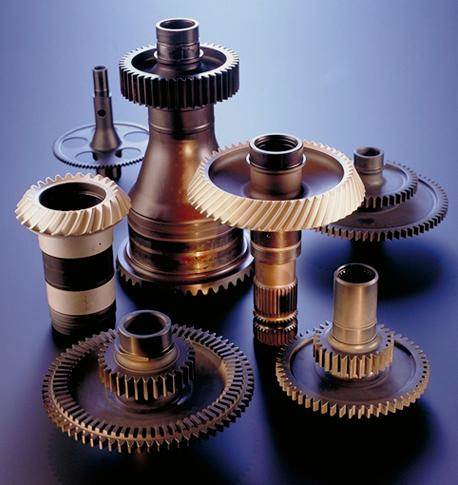
\includegraphics{figures/ch-00-example-pignon}}
  
  \caption{\label{fig:exemples-pieces}Exemples de pièces de transmission de puissance soumises à des traitements thermochimiques (source: Safran Group).}
\end{figure}

Le traitement de carbonitruration est un procédé thermochimique de traitement des matériaux qui, par l'introduction de carbone et d'azote à la surface des aciers, améliore les résistances à la fatigue et à l'usure des pièces traitées. Typiquement, la thermochimie du procédé peut être considérée comme la combinaison d'une cémentation et d'une nitruration dans le domaine austénitique, généralement dans la plage allant de \SIrange{1073}{1173}{\kelvin}~\cite{Slycke1981i,Slycke1981ii}. Bien que la pratique industrielle consiste le plus souvent en l'enrichissement simultané de l'alliage par les deux éléments interstitiels, les résultats présentés ici sont relatifs à un traitement de carbonitruration réalisé comme une séquence d'étapes de cémentation et de nitruration. Cette approche vise à explorer les réponses métallurgiques et mécaniques des alliages étudiés plutôt que les paramètres du procédé de carbonitruration~\cite{Slycke1981i,Sproge1988} et minimise la formation de composants toxiques comme les cyanures pendant le traitement. L'étude de la cinétique gazeuse du procédé se fait d'abord séparément et ses fondements seront abordées à la fin de ce chapitre.

Le plus souvent, le traitement de carbonitruration est effectué sur du fer pur, des aciers faiblement alliés à faible teneur en carbone et des pièces issues de la métallurgie des poudres. Le présent travail traite uniquement du comportement des aciers faiblement alliés. La faible teneur en carbone a pour rôle d'augmenter la cinétique du procédé \textendash{} augmentation du gradient de potentiel chimique entre la surface et le c{\oe}ur du matériau \textendash{} tout en maintenant la ténacité au c{\oe}ur des pièces. Les éléments d'alliage sont destinés à optimiser la trempabilité en surface, promouvoir le durcissement par solution solide à c{\oe}ur et favoriser la précipitation des carbures et nitrures lors du revenu. Comme les fractions d'interstitiels typiquement introduites en surface par le traitement thermochimique sont dans la gamme de fractions massiques allant de 0,005 à 0,007 (en considérant le carbone et/ou l'azote), typiquement une microstructure de martensite en lattes est obtenue dans le gradient de composition~\cite{Steel2006}. La présence d'éléments d'alliage, comme le chrome et le manganèse, implique un comportement différent de celui observé dans le système \ch{Fe-C-N}~\cite{vanGent1985,Mittemeijer1988} en raison de leurs effets sur la transformation martensitique, la résistance au revenu et la précipitation des nitrures à la température de traitement~\cite{Kaplow1983}, ce qui réduit de façon drastique la solubilité de l'azote dans l'austénite.

Le procédé exploite principalement la transformation martensitique pour obtenir les propriétés désirées dans les pièces traitées. Le traitement doit toujours être suivi d'une trempe afin de produire les résultats souhaités. Les contraintes introduites par la trempe dépassent~\footnote{Sur une profondeur qui dépend de la composition de la nuance, de la fraction en interstitiels et des conditions de transfert thermique du milieu de trempe.} l'énergie de déformation requise par la transformation martensitique~\cite{Khachaturyan1983}, ce qui conduit à une phase fragile avec des contraintes internes élevées.  Une dernière étape de revenu \textendash{} typiquement à une température de l'ordre de \SI{473}{\kelvin} \textendash{} est nécessaire pour augmenter la ténacité de la martensite pour les applications visées. Bien que le modèle de \citet{Norstrom1976}, qui sera utilisé dans l'analyse des réponses mécaniques, traduise assez bien le comportement en dureté de la martensite après trempe, les propriétés mécaniques des pièces traitées et revenues dépendent d'une série de mécanismes complexes qui seront abordés tout au long du texte. En outre, la nature des phases à l'équilibre à la température de revenu et leur cinétique de formation jouent un rôle important sur les propriétés finales des alliages qui peuvent s'établir dans des conditions de para--équilibre~\cite{Ghosh2001}.

À l'échelle du laboratoire, le procédé de carbonitruration a fait l'objet d'études à la fois à la pression atmosphérique et sous vide.  En effet, en raison de la maîtrise acquise à l'Institut Jean Lamour sur les processus interfaciaux se déroulant dans un procédé de thermogravimétrie fonctionnant à pression atmosphérique, il a été décidé de bénéficier de cette expérience pour comprendre le comportement métallurgique des nuances traitées, avant de procéder à un transfert des résultats obtenus dans ces conditions à des réacteurs opérant sous vide.

La caractérisation chimique et microstructurale des aciers traités a permis de mieux comprendre le comportement en diffusion-précipitation du carbone et plus spécialement de l'azote dans les deux alliages étudiés.  Le procédé à pression atmosphérique a également fait l'objet de diagnostics par chromatographie en phase gazeuse et par thermogravimétrie, afin de déterminer l'influence des processus de volume par rapport aux processus de surface lors de la décomposition des précurseurs et de l'enrichissement des nuances en carbone et en azote.

Pour la modélisation de l'enrichissement des alliages étudiés, le logiciel Thermo-Calc~\cite{Andersson2002,Borgenstam2000} a été employé~\footnote{L'édition 2015 de ce logiciel intègre déjà Dictra~\cite{Borgenstam2000} comme un module au lieu d'un programme séparé. Dans le texte, si l'on parle de simulation de diffusion avec Thermo-Calc~\cite{Andersson2002,Borgenstam2000}, cela veut dire l'emploi du module Dictra~\cite{Borgenstam2000}}. Ce logiciel permet de traiter la modélisation de la diffusion des éléments interstitiels et de la précipitation de nitrures et de carbures qui décrit les transformations à l'état solide. Les profils de diffusion ainsi obtenus sont comparés à des simulations en utilisant les interdépendances des diffusivités du carbone et de l'azote qui ont été proposées et validées par \citet{Slycke1981ii}. L'étude du comportement cinétique des atmosphères a été réalisée en utilisant un code développé dans les langages de programmation C++ et Python en utilisant les librairies TChem~\cite{Tchem2011} et Cantera~\cite{Cantera2014} pour le calcul des vitesses de réaction et CVode~\cite{Hindmarsh2005} pour l'intégration du système d'équations ainsi généré. Les librairies Boost~\cite{BoostGraph2001} et NetworkX~\cite{Networkx2016} ont été employées dans l'analyse des graphes chimiques permettant l'implémentation de la méthode de \citet{Lu2006i} pour la simplification des systèmes cinétiques et l'obtention de modèles compatibles avec des simulations couplées de la cinétique de décomposition des précurseurs et de l'hydrodynamique du réacteur.

Ce mémoire de thèse est divisé en trois parties: tout d'abord la Partie~\ref{part:part_1} contient une revue bibliographique et théorique des différentes avancées sur les traitements thermochimiques des aciers faiblement alliés. Ensuite, dans la Partie~\ref{part:part_2} est présentée une étude expérimentale des traitements thermochimiques et de la cinétique de décomposition des précurseurs utilisés. Enfin, la modélisation des procédés est traitée dans la Partie~\ref{part:part_3}. Cette thèse s'inscrit dans le cadre d'un partenariat de recherche entre différentes entités académiques et industrielles, réunies dans l'Institut de Recherche Technologique Matériaux, Métallurgie et Procédés (IRT M2P) autour du projet Traitements Thermochimiques Avancées. Les travaux de recherche ont été réalisés au sein de l'Institut Jean Lamour (IJL) à l'Université de Lorraine.

\endinput